\section{Preliminaries}\label{sec:DCCCs}

Here we recap \textit{dynamically condensed colour codes} (DCCCs) \cite{kesselring2022anyon} and how such codes can be used to detect and correct errors. DCCCs are a type of \textit{dynamic stabilizer code}. We refer those interested in a more general introduction to the latter topic to \Ccite{fu2024errorcorrectiondynamicalcodes, Townsend_Teague_2023}. We will assume the reader is comfortable with the stabilizer formalism.
Otherwise, we recommend \Ccite{NielsenChuang,GottesmanQECBook2024} for a basic introduction to this topic. 

DCCCs can be defined in terms of the colour code's \textit{boson table},
a $3 \times 3$ grid with columns labelled by colours $c, m$ and $y$ (cyan, magenta, and yellow)
and rows labelled by letters $X, Y$ and $Z$ (non-identity Pauli matrices).
Cells of the table are thus colour-Pauli pairs $(\kappa, P)$.
Often we will want to talk about generic colours $\{\kappa, \kappa', \kappa''\} = \{c, m, y\}$
and generic Pauli matrices $\{P, P', P''\} = \{X, Y, Z\}$,
for which we will use a boson table with these generic labels instead:
\begin{equation}\label{eq:cc_boson_table}
\bosonTable{
    rx={\colourful{c}, X},
    gx={\colourful{m}, X},
    bx={\colourful{y}, X},
    ry={\colourful{c}, Y},
    gy={\colourful{m}, Y},
    by={\colourful{y}, Y},
    rz={\colourful{c}, Z},
    gz={\colourful{m}, Z},
    bz={\colourful{y}, Z},
}
\qquad \text{or} \qquad
\bosonTable{
    rx={\kappa, P},
    gx={\kappa', P},
    bx={\kappa'', P},
    ry={\kappa, P'},
    gy={\kappa', P'},
    by={\kappa'', P'},
    rz={\kappa, P''},
    gz={\kappa', P''},
    bz={\kappa'', P''},
}
\end{equation}

A DCCC can be defined on any three-face-colourable, three-valent 2D lattice.
Edges of such a lattice inherit a canonical colouring;
an edge separating faces of colours $\kappa$ and $\kappa'$ is assigned the third colour $\kappa''$.
On every vertex of the lattice we place a qubit.
Throughout this work we use the honeycomb lattice.
We also assume throughout that this lattice is placed on a torus;
we comment on the limitations of this in \Cref{subsec:boundaries}.

For every cell $(\kappa, P)$ of the boson table, we can define certain operators on the lattice.
Namely, for every $\kappa$-coloured edge $e_\kappa = (v_0, v_1)$,
we can define a \textit{$(\kappa, P)$ edge operator} $\dcccOp{e}{\kappa}{P} \defeq P_{v_0} P_{v_1}$,
and the set of all such edge operators as $\dcccOp{E}{\kappa}{P}$.
Similarly, for every $\kappa$-coloured face $f_\kappa$ with vertices $v_0, v_1, \ldots, v_5$
we can define a \textit{$(\kappa, P)$ face operator} $\dcccOp{f}{\kappa}{P} \defeq P_{v_0} P_{v_1} \ldots P_{v_5}$,
and the set of all such face operators as $\dcccOp{F}{\kappa}{P}$. 
Note that each face operator $\dcccOp{f}{\kappa}{P}$ can be made from edge operators in two ways; as the product of the three $(\kappa', P)$ edge operators around $f$, or the three $(\kappa'', P)$ edge operators.
Additionally, it can be written as the product of the other two face operators $\dcccOp{f}{\kappa}{P'}$ and $\dcccOp{f}{\kappa}{P''}$ on $f$, up to global phase.
Examples of such operators are shown in \Cref{fig:edge_and_face_operator}.

\begin{figure}[htbp!]
    \centering
     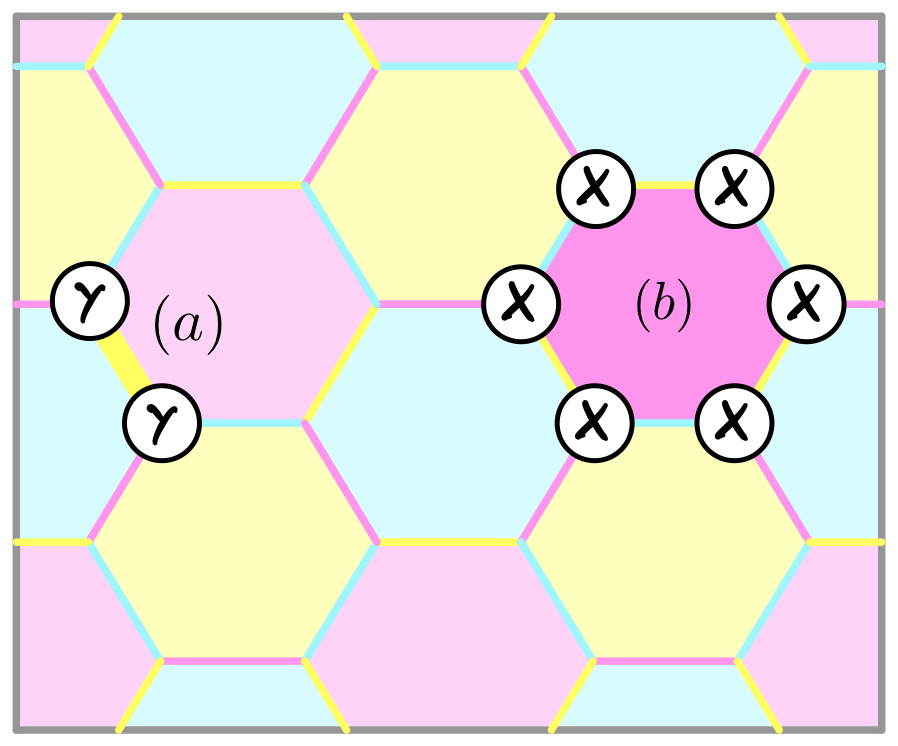
\includegraphics[width=180pt]{figures/DCCCs/edge_and_face_operator}
    \caption{
        $(a)$ A $Y^{\otimes 2}$ yellow edge operator $e_{\textcolor{Dandelion}{y}, {Y}}$.
        $(b)$ An $X^{\otimes 6}$ magenta face operator $f_{\textcolor{magenta}{m}, {X}}$.
    }
    \label{fig:edge_and_face_operator}
\end{figure}

\subsection{Measurement schedule}\label{subsec:measurement_schedule}

A DCCC, then, is a dynamic stabilizer code defined by
repeatedly measuring sets $\dcccOp{E}{\kappa}{P}$ of all $(\kappa, P)$ edge operators.
We say it has \textit{measurement schedule} $\left(
    \langle \dcccOp{E}{\kappa_0}{P_0} \rangle,
    \langle \dcccOp{E}{\kappa_1}{P_1} \rangle,
    \ldots
    \right)$.
For DCCCs as defined in \Ccite[Section 7]{kesselring2022anyon}, there is a single restriction:
if at time $t$ the operators $\dcccOp{E}{\kappa_t}{P_{t}}$ are measured,
then at time $t+1$ we must choose a new set $\dcccOp{E}{\kappa_{t+1}}{P_{t+1}}$ of edges to measure,
such that cell $(\kappa_{t+1}, P_{t+1})$ shares neither a row nor column with $(\kappa_t, P_t)$ in the boson table.
Later, in \Cref{sec:gauge_dcccs}, we relax this restriction and investigate DCCCs with repeated measurements -- i.e. we allow $\dcccOp{E}{\kappa_{t+1}}{P_{t+1}} = \dcccOp{E}{\kappa_t}{P_t}$.
But until then, the two DCCCs we will focus on are
the \textit{$X^1Y^1Z^1$ honeycomb code} from \Ccite{hastings2021dynamically} and the \textit{$X^1Z^1$ honeycomb code} from 
\Ccite{kesselring2022anyon} \footnote{The $X^1Y^1Z^1$ honeycomb code is equivalent to the Hastings-Haah code up to conjugating certain qubits by Cliffords.}. 


These are defined by the measurement schedules
\begin{equation}\label{eq:honeycomb_codes_measurement_schedules}
    \begin{aligned}
        \MMM_{X^1Y^1Z^1} &= \left(
            \langle \dcccOp{E}{c}{X} \rangle,
            \langle \dcccOp{E}{m}{Y} \rangle,
            \langle \dcccOp{E}{y}{Z} \rangle
        \right),\\
        \MMM_{X^1Z^1} &= \left(
            \langle \dcccOp{E}{c}{X} \rangle,
            \langle \dcccOp{E}{m}{Z} \rangle,
            \langle \dcccOp{E}{y}{X} \rangle,
            \langle \dcccOp{E}{c}{Z} \rangle,
            \langle \dcccOp{E}{m}{X} \rangle,
            \langle \dcccOp{E}{y}{Z} \rangle
        \right).
    \end{aligned}
\end{equation}
Much of this work is concerned with the properties of these two codes and their performances under different noise models and decoders.

\begin{figure}[h!]
    \centering
    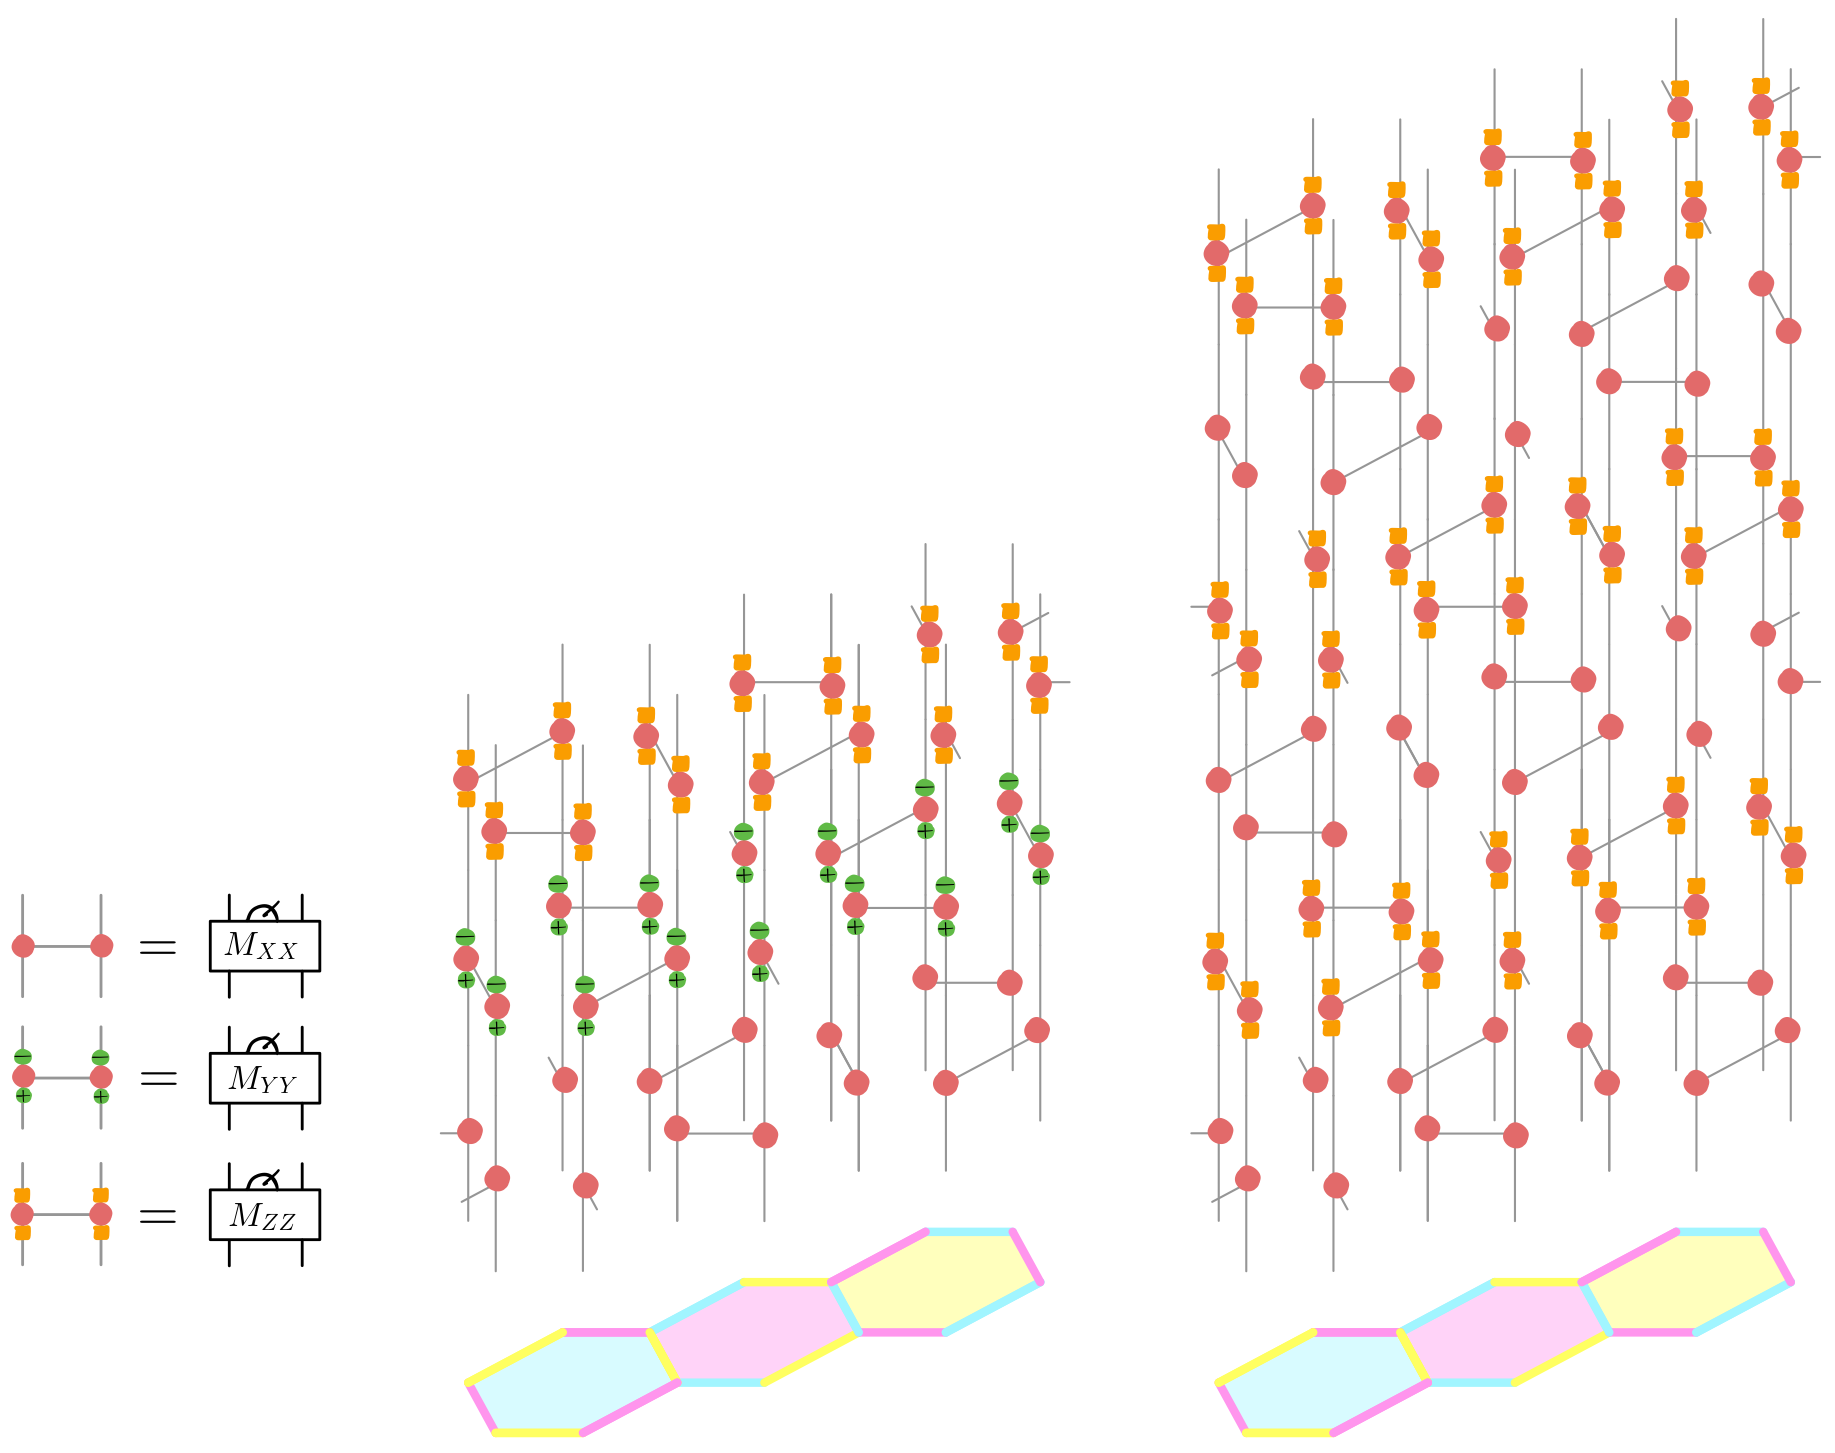
\includegraphics[width=400pt]{figures/DCCCs/schedules_XYZ_and_CSS_measurements_next_to}
    \caption{
        For a subset of qubits, we show the sequence of measurements defining the $X^1 Y^1 Z^1$ (middle) and $X^1 Z^1$ (right) honeycomb codes.
        This figure uses the ZX-calculus~\cite{Coecke_2011}, a rigorous graphical language for quantum mechanics.
        For those unfamiliar with the ZX-calculus, a crash course is given in \Cref{sec:zx-calculus-and-pauli-webs},
        with proper introductions available in \Ccite{vandewetering2020zxcalculusworkingquantumcomputer,KissingerWetering2024Book}.
        Alternatively, you're absolutely free to ignore these diagrams' rigorous meaning and treat them as a visual guide to the algebra in the text -- much in the same way as \Cref{fig:edge_and_face_operator} has no rigorous meaning.
        In which case, all you need to know for now is that the diagrams are read bottom-to-top and the three diagrams on the left of the figure denote measurements of $X \otimes X$, $Y \otimes Y$ and $Z \otimes Z$ respectively.
    }
    \label{fig:schedules_XYZ_and_CSS}
\end{figure}

\subsection{Stabilizers and logical operators}\label{subsec:stabilizer_and_logicals}

\begin{figure}[b]
    \centering
    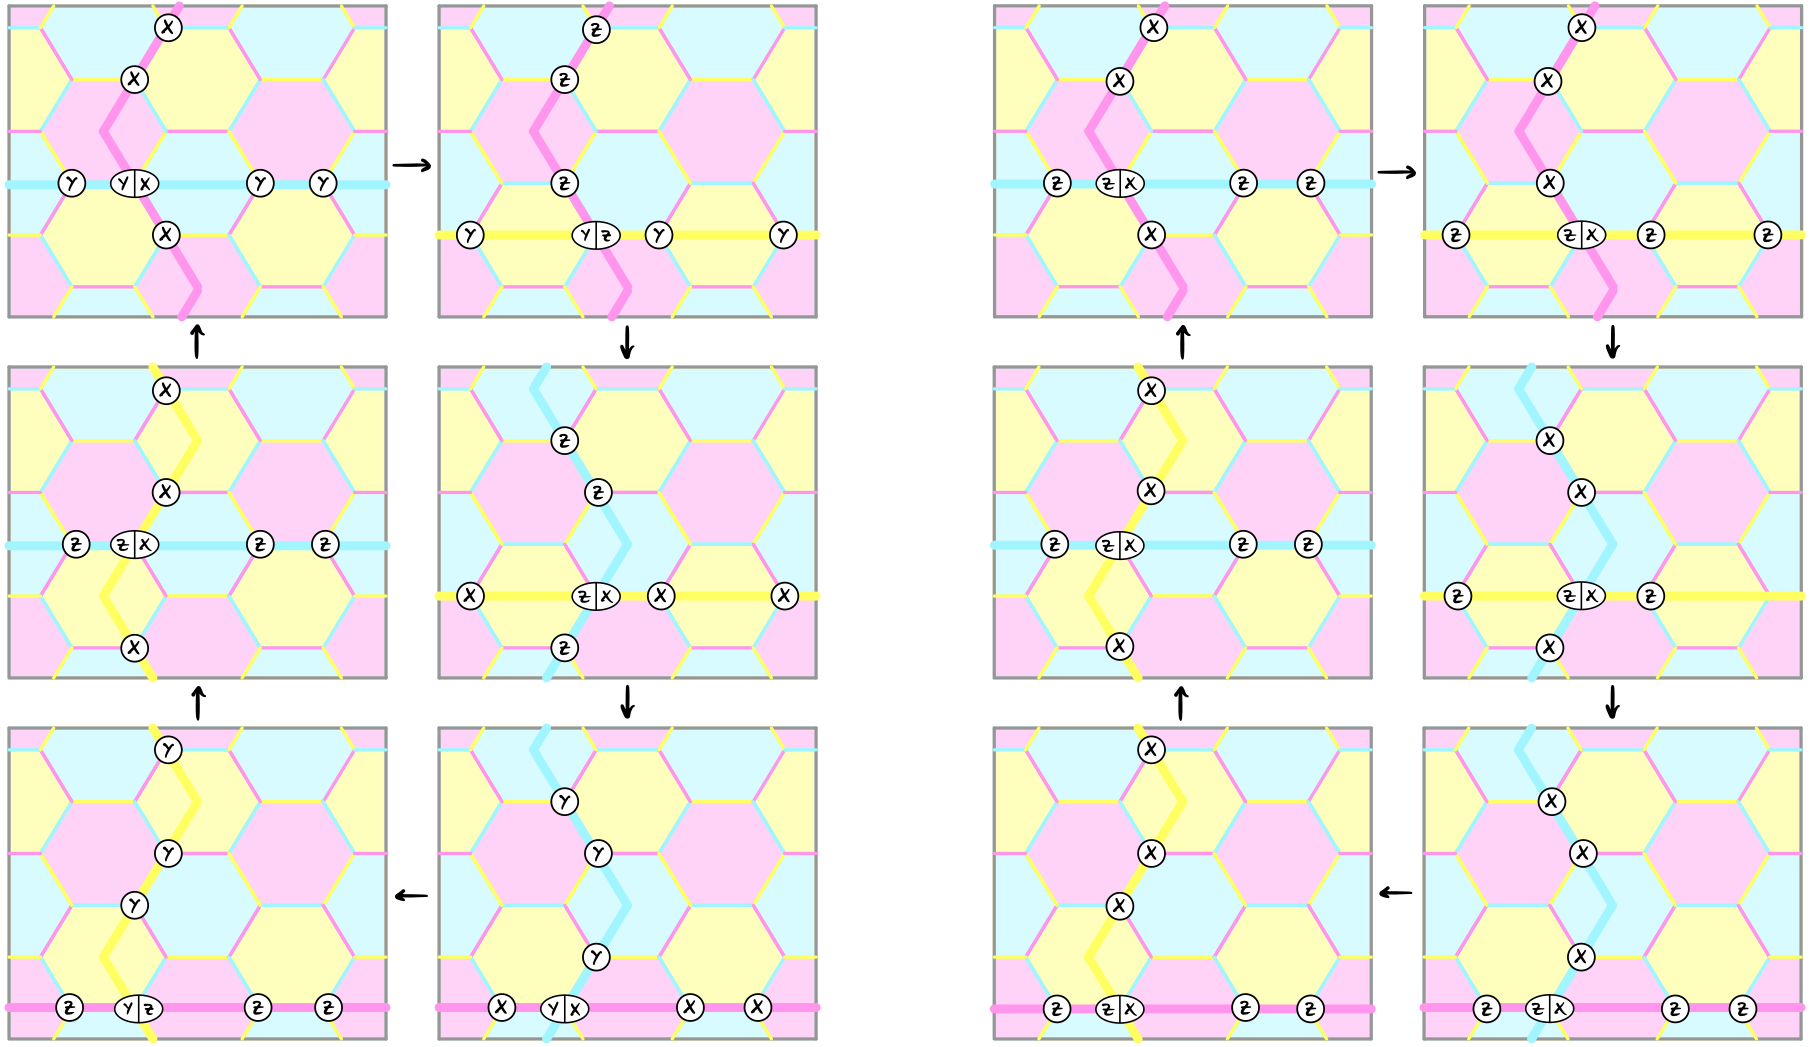
\includegraphics[width=\linewidth]{figures/DCCCs/logicals_XYZ_and_XZ_stacked_horizontal}
    \caption{
        Representatives of logical $E$ and $M$ operators for the $X^1 Y^1 Z^1$ (left) and $X^1 Z^1$ (right) honeycomb codes at timesteps $t$ mod $6$.
        Timestep $0$ mod $6$ is the top left subfigure in each cycle.
        Boundaries are periodic, forming a torus.
        Throughout this work we say a DCCC encodes only one logical qubit - we just ignore the other one.
        We arbitrarily choose that the $E$ logical operator wraps vertically around the torus in this figure, with the $M$ operator wrapping around horizontally.
        Importantly, the representative of the $E$ operator in the $X^1 Z^1$ code always consists of Pauli $Z$ operators, and the $M$ operator always consists of Pauli $X$ operators.
        In the $X^1 Y^1 Z^1$ code, in contrast, the representatives of both the $E$ and $M$ operator consist one third of the time of Pauli $X$ operators, one third of the time of $Y$ operators and one third of the time of $Z$ operators.
        This will be important when discussing the effects of biased noise later on.}
    \label{fig:logicals_XYZ_and_XZ}
\end{figure}

In any dynamic stabilizer code on $n$ qubits, once a measurement schedule has been defined, two further sequences can be derived;
the \textit{instantaneous stabilizer groups} (ISGs) $\SSS = (\SSS_{-1}, \SSS_0, \SSS_1, \ldots)$
and the \textit{instantaneous logical Pauli groups} (ILPGs) $\LLL = (\LLL_{-1}, \LLL_0, \LLL_1, \ldots)$.
These respectively track -- at each timestep $t$ -- which Paulis are stabilizers of our code,
and which Paulis are representatives of logical Pauli operators.
Explicit presentations for each $\SSS_t$ and $\LLL_t$ can be found via the stabilizer formalism \cite[Section 6.2]{GottesmanQECBook2024}.
We let $r_t$ denote the rank of $\SSS_t$.
The group $\LLL_t$ is defined to be $\lpglong{t}$, the normaliser of $\SSS_t$ in the Pauli group, modulo $\SSS_t$.
Every $\LLL_t$ is isomorphic to the Pauli group $\PPP_{k_t}$ on $k_t \coloneq n - r_t$ qubits~\cite[Theorem 3.11]{GottesmanQECBook2024}.
If there is a timestep $T$ such that for all $t \geq T$ we have $r_t = r_T \eqqcolon r$, then we say the code is \textit{established}.
Correspondingly, for such $t \geq T$, we get $k_{t} = k_T \eqqcolon k$.
We thus say such a code encodes $k$ logical qubits.

Every DCCC on a torus has an establishment time $T$, after which it encodes $k=2$ logical qubits.
Alternatively, we can always just ignore one of the logical qubits and pretend it only encodes one qubit; this makes our work more straightforward to compare with the more easily implementable planar case, which encodes just one logical qubit, and allows us to tailor the code dimensions to biased noise models later on.
In the rest of this work, we will do exactly this.
In \Cref{fig:logicals_XYZ_and_XZ}, we show representatives of logical $X$ and $Z$ operators for the $X^1Y^1Z^1$ and $X^1Z^1$ honeycomb codes at timesteps $t$ mod $6$.
For reasons we discuss shortly (\Cref{subsec:E_and_M_components}), we will actually call these $E$ and $M$ logical operators rather than $X$ and $Z$.

\subsection{Noise models}\label{subsec:noise_models}

Before we can discuss how DCCCs are used to detect and correct errors, we need to meet the errors in question.

\subsubsection{Direct parity measurement noise model}
In a quantum circuit that implements a DCCC -- one that repeatedly performs the defining sequence of measurements $\MMM = (\groupPres{\dcccOp{E}{\kappa_0}{P_0}}, \groupPres{\dcccOp{E}{\kappa_1}{P_1}}, \ldots)$ --
in addition to the $n$ \textit{data qubits},
we may require additional \textit{auxiliary qubits} in order to perform the measurements.
In the \textit{direct parity measurement noise model},
we assume that two-qubit parity measurements (such as $XX$, $YY$, $ZZ$) can be performed natively.
We assume that at every timestep $t$,
before a generating set for $\MMM_t$ is measured,
any of the $n$ data qubits can be afflicted by a single-qubit Pauli error $X$, $Y$, or $Z$ with probability $p_X$, $p_Y$, or $p_Z$ respectively.
We call these \textit{data qubit errors}.
We also assume that every measurement can be erroneously reported with probability $p_m$ --
i.e.\ the actual measurement outcome is $\pm 1$, but the reported measurement outcome is $\mp 1$.
We call this a \textit{measurement error}, or \textit{measurement noise}.
A noise model is \textit{biased} unless all of these probabilities are equal.
Tailoring DCCCs to be effective against biased noise models will be a key theme of this work.
The two types of bias we will focus on are \textit{measurement bias} and \textit{$Z$ bias}.
In the direct parity measurement noise model, the measurement bias is defined as
$\eta_m = p_m/(p_X + p_Y + p_Z)$,
and the $Z$ bias is defined as
$\eta_Z = 2p_Z/(p_X+p_Y)=p_Z/p_X$, assuming $p_X=p_Y$.

In any circuit we keep the total physical error rate $p$ fixed as
\begin{equation}\label{eq:physical_error_rate_defn}
    p = \frac{p_m M + (p_X + p_Y + p_Z) Q} {M + 3Q}
\end{equation}
where $M$ is the number of measurements in the circuit and $Q$ is the number of data qubit noise locations.
To generate 
\Cref{fig:phenomenological_noise_volume_plot_beliefmatching,fig:phenomenological_noise_volume_plot_pymatching}, we have used $p = 10^{-3}$.


\begin{figure}[p]
  \centering
    \begin{subfigure}[c]{0.14\textwidth}
        \centering
        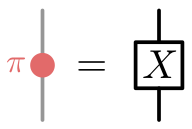
\includegraphics[width=0.8\textwidth]{figures/DCCCs/ZX_X_gate}
        \caption{}
        \label{fig:ZX_X_gate}
    \end{subfigure}
    \begin{subfigure}[c]{0.14\textwidth}
        \centering
        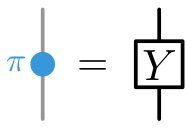
\includegraphics[width=0.8\textwidth]{figures/DCCCs/ZX_Y_gate}
        \caption{}
        \label{fig:ZX_Y_gate}
    \end{subfigure}
    \begin{subfigure}[c]{0.14\textwidth}
        \centering
        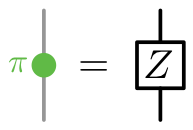
\includegraphics[width=0.8\textwidth]{figures/DCCCs/ZX_Z_gate}
        \caption{}
        \label{fig:ZX_Z_gate}
    \end{subfigure}
    \begin{subfigure}[c]{0.27\textwidth}
        \centering
        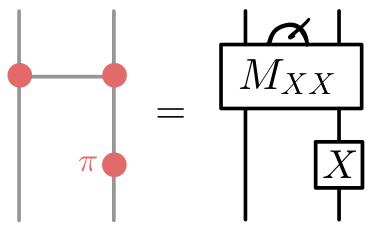
\includegraphics[width=0.8\textwidth]{figures/DCCCs/ZX_XX_meas_X_error}
        \caption{}
        \label{fig:ZX_XX_meas_X_error}
    \end{subfigure}
    \begin{subfigure}[c]{0.27\textwidth}
        \centering
        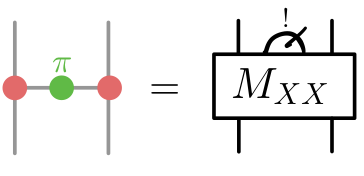
\includegraphics[width=0.8\textwidth]{figures/DCCCs/ZX_XX_meas_error}
        \caption{}
        \label{fig:ZX_XX_meas_error}
    \end{subfigure}
    \caption{
        Subfigures (a), (b) and (c) show the non-identity Pauli gates as ZX-diagrams.
        Subfigures (d) and (e) show examples of errors in a phenomenological noise model.
        Specifically, (d) shows an $X$ error occurring before an $e_{\kappa, X}$ measurement,
        while (e) shows a measurement error on an $e_{\kappa, X}$ measurement.
        Indeed, throughout this work, a measurement error on any $e_{\kappa, P}$ measurement will correspond in the ZX-calculus to a two-legged green $\pi$-spider on a `horizontal' wire.
    }
    \label{fig:phenom_error_examples}

    \vspace{20pt}
  
  \begin{subfigure}[b]{0.2\textwidth}
        \centering
        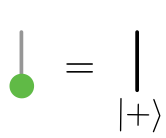
\includegraphics[width=0.6\textwidth]{figures/DCCCs/ZX_plus_init}
        \caption{}
        \label{fig:ZX_plus_init}
    \end{subfigure}
    \begin{subfigure}[b]{0.2\textwidth}
        \centering
        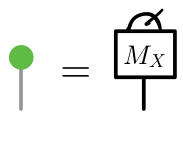
\includegraphics[width=0.6\textwidth]{figures/DCCCs/ZX_X_meas}
        \caption{}
        \label{fig:ZX_X_meas}
    \end{subfigure}
    \begin{subfigure}[b]{0.3\textwidth}
        \centering
        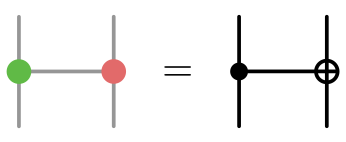
\includegraphics[width=0.7\textwidth]{figures/DCCCs/ZX_CNOT}
        \caption{}
        \label{fig:ZX_CNOT}
    \end{subfigure}
    \begin{subfigure}[b]{0.45\textwidth}
        \centering
        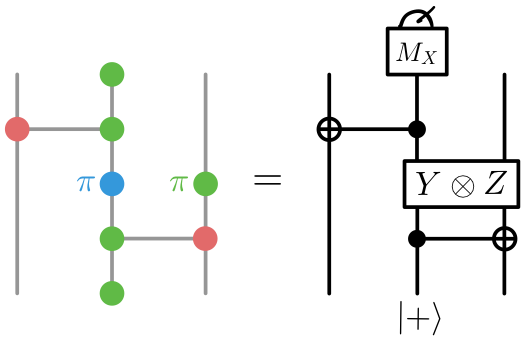
\includegraphics[width=0.7\textwidth]{figures/DCCCs/ZX_XX_meas_circuit_YZ_error}
        \caption{}
        \label{fig:ZX_XX_meas_circuit_YZ_error}
    \end{subfigure}
    \begin{subfigure}[b]{0.45\textwidth}
        \centering
        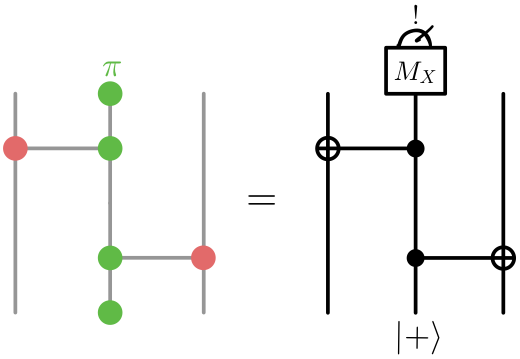
\includegraphics[width=0.7\textwidth]{figures/DCCCs/ZX_XX_meas_circuit_meas_error}
        \caption{}
        \label{fig:ZX_XX_meas_circuit_meas_error}
    \end{subfigure}
    \caption{
        Subfigures \textbf{(a)}, \textbf{(b)} and \textbf{(c)} show the $\ket{+}$ state, $X$ measurement and $CX$ gate respectively as ZX-diagrams.
        Subfigures \textbf{(d)} and \textbf{(e)} show examples of errors in an auxiliary qubit circuit noise model,
        where two-qubit gates and a single-qubit measurement are used to measure $e_{\kappa, X}$.
        Specifically, \textbf{(d)} shows a $Y \otimes Z$ error occurring immediately after a $CX$ gate,
        while \textbf{(e)} shows a measurement error on an $X$ measurement.
    }
    \label{fig:circuit_level_error_examples}

    \vspace{20pt}
  
    \begingroup
    \renewcommand*{\arraystretch}{1.2}
        \centering
        \begin{tabular}{|p{30mm}|p{60 mm}|p{10mm}|p{10mm}|p{10mm}|}
            \hline
            Operation & Noise applied after operation & SD & SI & EM3 \\
            \hline
            \hline
             CX, CY, CZ & $\{I,X,Y,Z\}^{\otimes 2} - \{I \otimes I\}$ & $p$ & $p$ & -  \\
            \hline
            Init. $\ket{+}$ & $Z$ & $p$ & $2p$ & $p$ \\
            Init. $\ket{i}$ & $Y$ & $p$ & $2p$ & $p$ \\
            Init. $\ket{0}$ & $X$ & $p$ & $2p$ & $p$ \\
            \hline
            Meas. $X, Y, Z$ & bit-flip &  $p$ & $5p$ & $p$ \\
            \hline
            Idle & $X,Y,Z$ & $p$ & $p/10$ & $p$ \\
            \hline
            Resonator idle* & $X,Y,Z$ & 0 & $2p$ &$0$ \\
            \hline
        $M_{PP}$** & $\{I, X, Y, Z\}^{\otimes 2} \times $ \{bit-flip, no-flip\} & - & - & $p$ \\
    
        \hline
    
        \end{tabular}
        \captionof{table}{Exact details of the noise models used for numerical simulations. The leftmost column contains all types of operations that are applied in the circuits. The second column lists which errors can occur after a gate. If multiple errors are given, one is chosen uniformly at random. 
        *Resonator idle refers to a circuit location during which a qubit is not measured or reset in a time step during which other qubits are being measured or reset. **With the $M_{PP}$ operation the two-qubit Pauli errors are applied before the measurement.}
        \label{tab:noise_table}
    \endgroup
\end{figure}

\subsubsection{Auxiliary qubit circuit noise model}

An \textit{auxiliary qubit circuit noise model} decomposes multi-qubit measurements into elementary gates using auxiliary qubits, in contrast to the direct parity measurement noise model which assumes native two-qubit parity measurements.
In an auxiliary qubit circuit noise model,
we ignore the distinction between data and auxiliary qubits.
Instead, we just assume that after every gate $g$ on $q$ qubits, any weight-$q$ Pauli operator can occur on these qubits with some probability $p_g$.
We continue to assume that measurement noise can occur.
At this point, the actual circuits used to implement the DCCCs become relevant.
We consider two different families of circuits, \emph{single-qubit measurement circuits} and \emph{two-qubit measurement circuits}.
In the first, the measurements of edge operators $\dcccOp{e}{\kappa}{P}$ are implemented via auxiliary qubits, two-qubit gates, and single-qubit Pauli measurements.
In the second, the measurements of edge operators are implemented `natively' -- no auxiliary qubits are used.

The single-qubit measurement circuits are simulated with two different auxiliary qubit circuit noise models: \textit{standard depolarizing} (SD) and \textit{superconducting-inspired} (SI).
The SI model is taken from \Ccite{gidney2021fault}. 
There is a slight difference between our SI model and \textit{SI1000} in \Ccite{gidney2021fault}, namely that in the SI1000 noise model it is assumed that the only two-qubit gate used is $CZ$, while the circuits here contain $CX$, $CY$, and $CZ$ gates.
The two-qubit measurement circuits are simulated with a different auxiliary qubit circuit noise model referred to as \textit{entangling measurements} (EM) noise.
The EM noise model is exactly the EM3 model taken from \Ccite{gidney2022benchmarking}.
The different gates, errors, and probabilities of each model are shown in \Cref{tab:noise_table}.

\subsection{Detectors}\label{subsec:detectors}

We detect and correct errors using \textit{detectors}
\cite{Gidney2021stimfaststabilizer,derks2024}.
A detector is a set of measurement outcomes $\{m_1, \ldots, m_b\}$ whose product is deterministic in the absence of noise.
In a stabilizer code, detectors are particularly simple;
they consist of the outcomes of measuring the same stabilizer twice at consecutive timesteps. In dynamic stabilizer codes, we will not necessarily measure the same operators at consecutive timesteps,
so detectors can look more complicated. 
However, they are still easy to find using the stabilizer formalism;
one is created anytime we measure a Pauli operator $p$ such that
$p$ or $-p$ is a stabilizer for the code at a particular timestep.
If we ever find that the product $m_1 \ldots m_b$ differs from the expected value,
then we can conclude that some errors must have affected our system.
We say that such a detector has been \textit{violated} by these errors.
% and we say that the detectors violated by a set of errors are the \textit{syndrome} of these errors.
Often we'll write a detector $\{m_1, \ldots, m_b\}$ as a formal product $m_1 \ldots m_b$ with powers taken mod 2.\footnote{%
    By formal product, we mean we forget that symbols like $m_j$ are actually stand-ins for values $-1$ and $1$,
    and treat the symbols just as objects to be moved around algebraically.
    By taking powers mod 2, we mean -- for example -- the formal product $m^3$ is the same as $m^1 =  m$.
    It seems only ${\sim}16.7\%$ of the authors of this work think formal products are the best way to write detectors.
    If you prefer linear algebra,
    you can also think of a detector as a binary vector -- see \Ccite{derks2024}.
    Or you can continue to just think of them as sets of measurement outcomes.}

Let's now look at DCCC detectors.
We let $m_t(\dcccOp{e}{\kappa_t}{P_t})$ denote
the outcome of measuring the edge operator $\dcccOp{e}{\kappa_t}{P_t}$ at time $t$,
and let $e \in f$ mean edge $e$ borders face $f$.
DCCCs have detectors\footnote{%
    This statement only holds if we make a distinction between detectors and \textit{observables}.
    An observable here doesn't have the usual meaning of a self-adjoint operator.
    Instead it refers to a special detector that's used to test whether the decoder correctly decoded the errors in a circuit~\cite{Gidney2021stimfaststabilizer,derks2024}.
    There are indeed observables that are not of this form.}
of the form $d = \prod_{t \in \tau} \prod_{e_{\kappa_t} \in f_{\kappa}} m_t(\dcccOp{e}{\kappa_t}{P_t})$
for some set of timesteps $\tau$ and some $\kappa$-coloured face $f_\kappa$.
For example, on the left of \Cref{fig:detectors_XYZ_and_CSS} we show a detector in the $XYZ$ honeycomb code,
and on the right a detector in the CSS honeycomb code,
both associated to some yellow face $f_{\colourful{y}}$.
As a formal product, with timesteps taken modulo 6, the former is written as
\begin{equation}\label{eq:XYZ_detector_yellow}
    \prod_{e_{\colourful{m}} \in f_{\colourful{y}}} m_4(\dcccOp{e}{m}{Y})
    \prod_{e_{\colourful{c}} \in f_{\colourful{y}}} m_3(\dcccOp{e}{c}{X})
    \prod_{e_{\colourful{m}} \in f_{\colourful{y}}} m_1(\dcccOp{e}{m}{Y})
    \prod_{e_{\colourful{c}} \in f_{\colourful{y}}} m_0(\dcccOp{e}{c}{X}),
\end{equation}
while the latter is
\begin{equation}\label{eq:CSS_detector_yellow}
    \prod_{e_{\colourful{m}} \in f_{\colourful{y}}} m_4(\dcccOp{e}{m}{X})
    \prod_{e_{\colourful{c}} \in f_{\colourful{y}}} m_0(\dcccOp{e}{c}{X}).
\end{equation}

\begin{figure}[t]
    \centering
    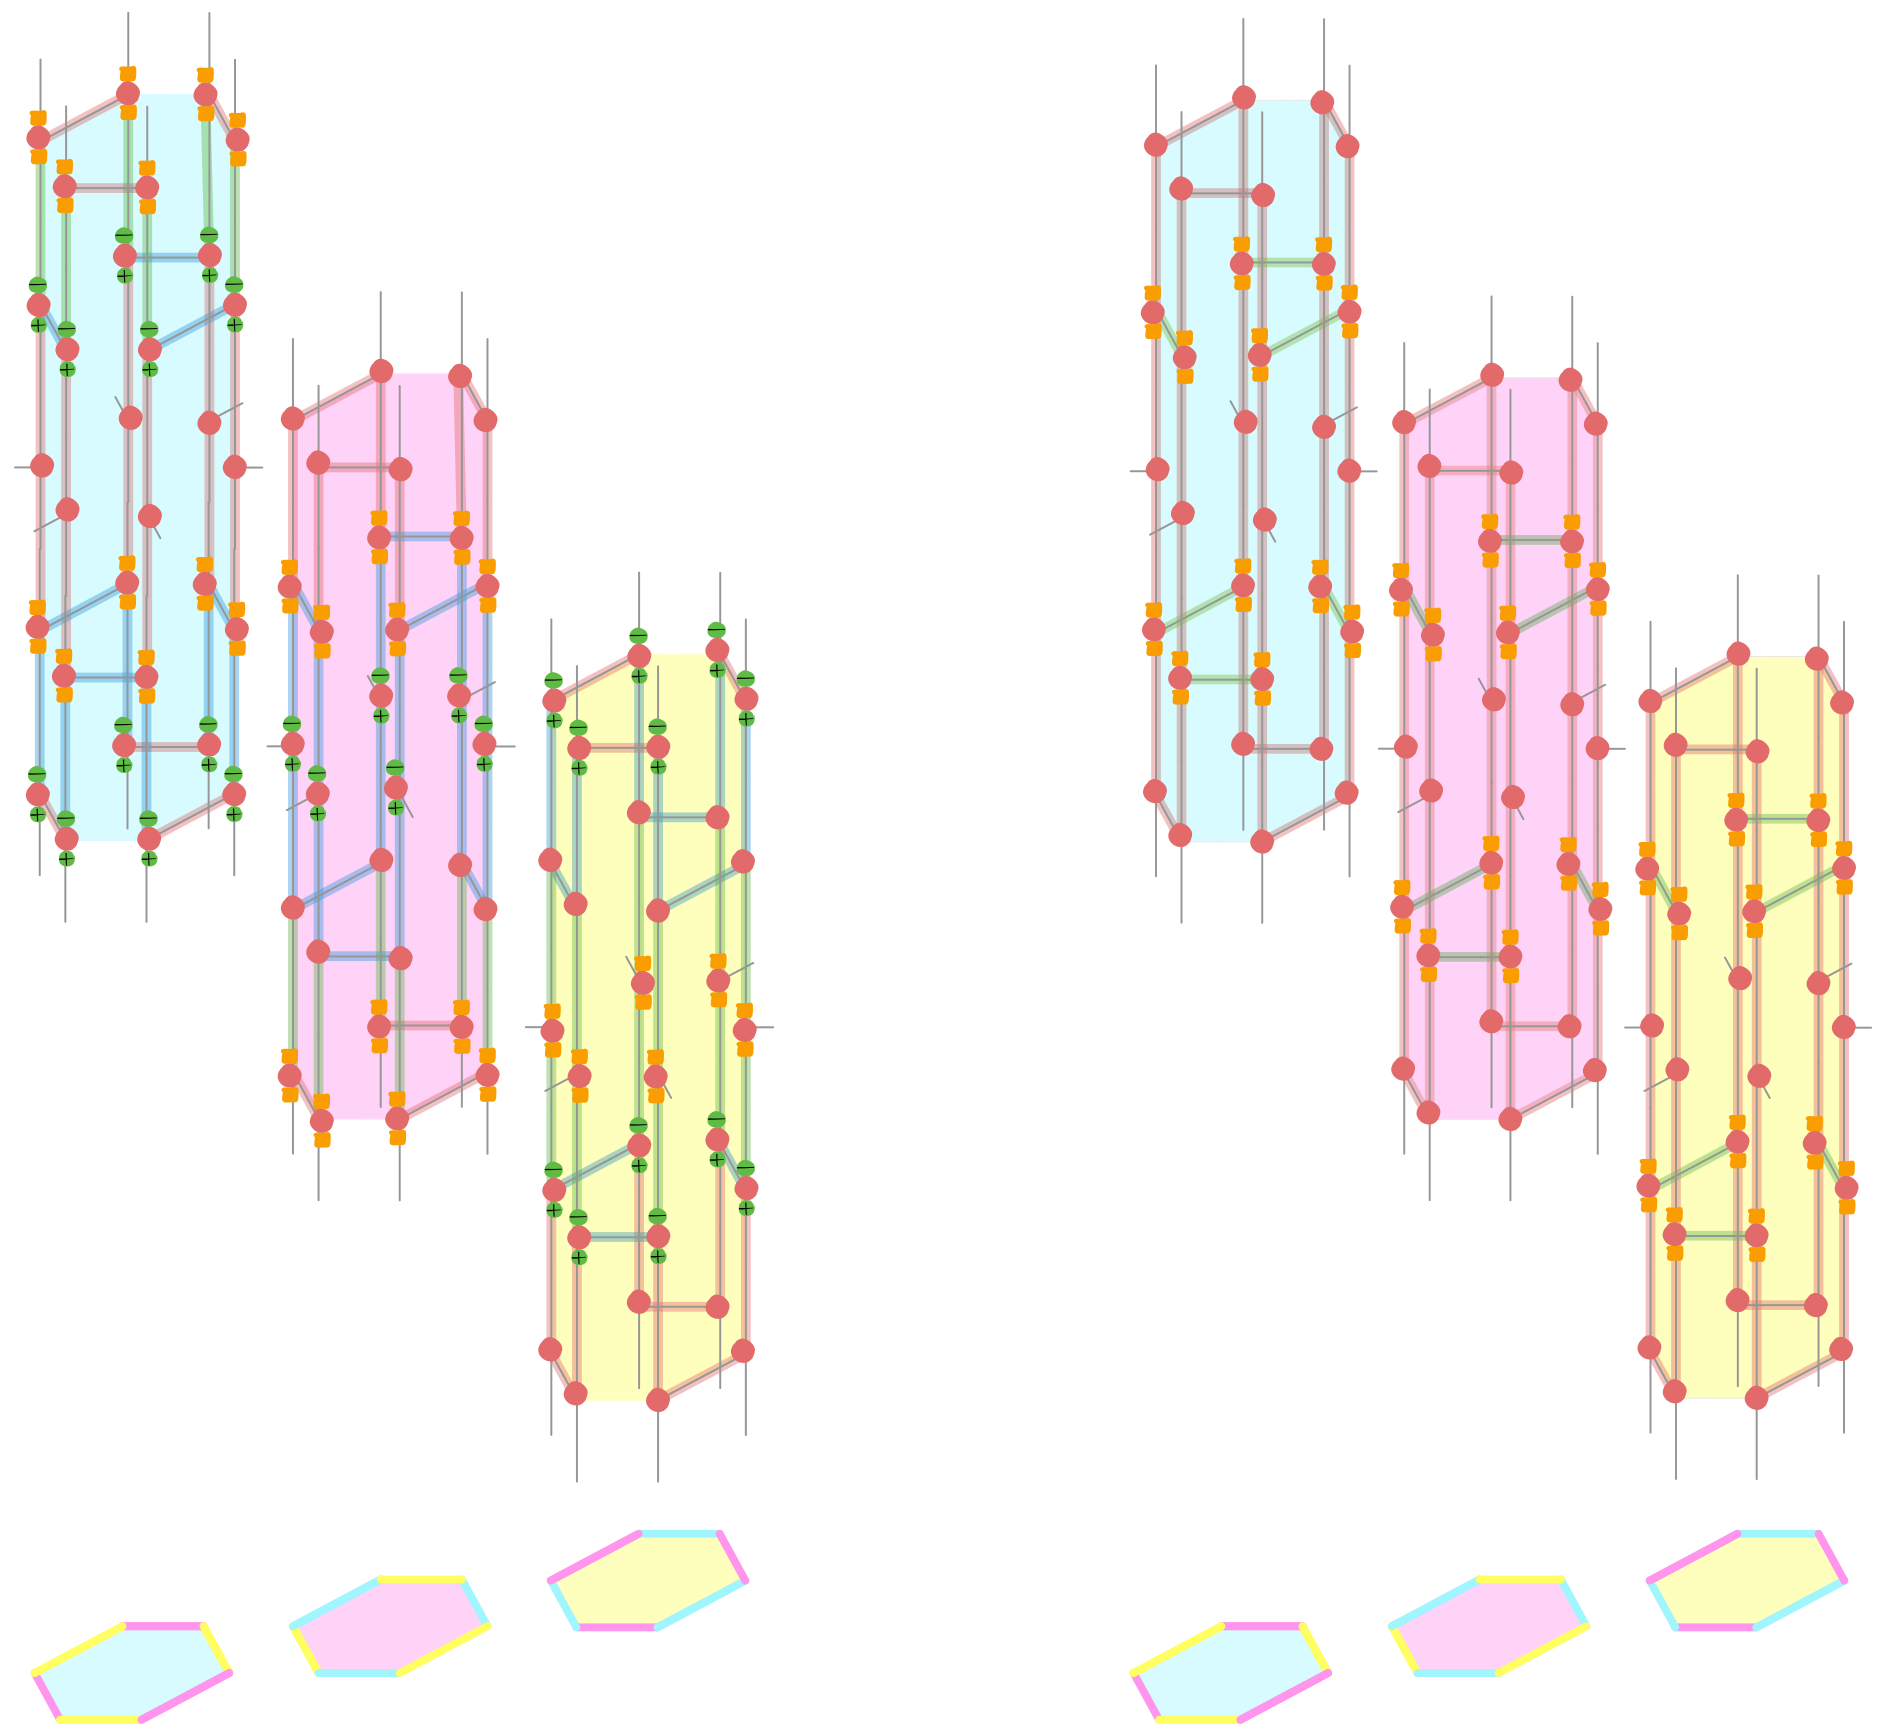
\includegraphics[width=0.8\linewidth]{figures/DCCCs/detectors_XYZ_and_CSS}
    \caption{
        A subset of detectors of the $X^1 Y^1 Z^1$ code (left) and the $X^1 Z^1$ code (right).
        Certain wires in this ZX-diagram are highlighted red, green or blue;
        they constitute a \textit{Pauli web}, which we go into in more detail in \Cref{sec:zx-calculus-and-pauli-webs}.
        In essence, one can think of a Pauli web as telling us which types of errors violate this detector at which timesteps.
        Pauli errors and measurement errors are represented in the ZX-calculus as 2-legged $\pi$-spiders (\Cref{fig:phenom_error_examples,fig:circuit_level_error_examples}).
        A detector is violated by a set of errors if there's an odd number of them of a different colour to the highlighted wire they sit on (see \Cref{fig:XYZ_measurement_error}, for example).
        Pauli webs also tell us which measurements are actually involved in a detector and which are not; it's all mesurements corresponding to non-vertical edges highlighted red or blue.
    }
    \label{fig:detectors_XYZ_and_CSS}
\end{figure}

In \Cref{fig:detectors_XYZ_and_CSS} the detectors are shown graphically via \textit{Pauli webs}, as explained in more detail in the caption.

\subsection{Decoding graph}\label{subsec:decoding_graph}

\begin{figure}[htbp]
    \centering
    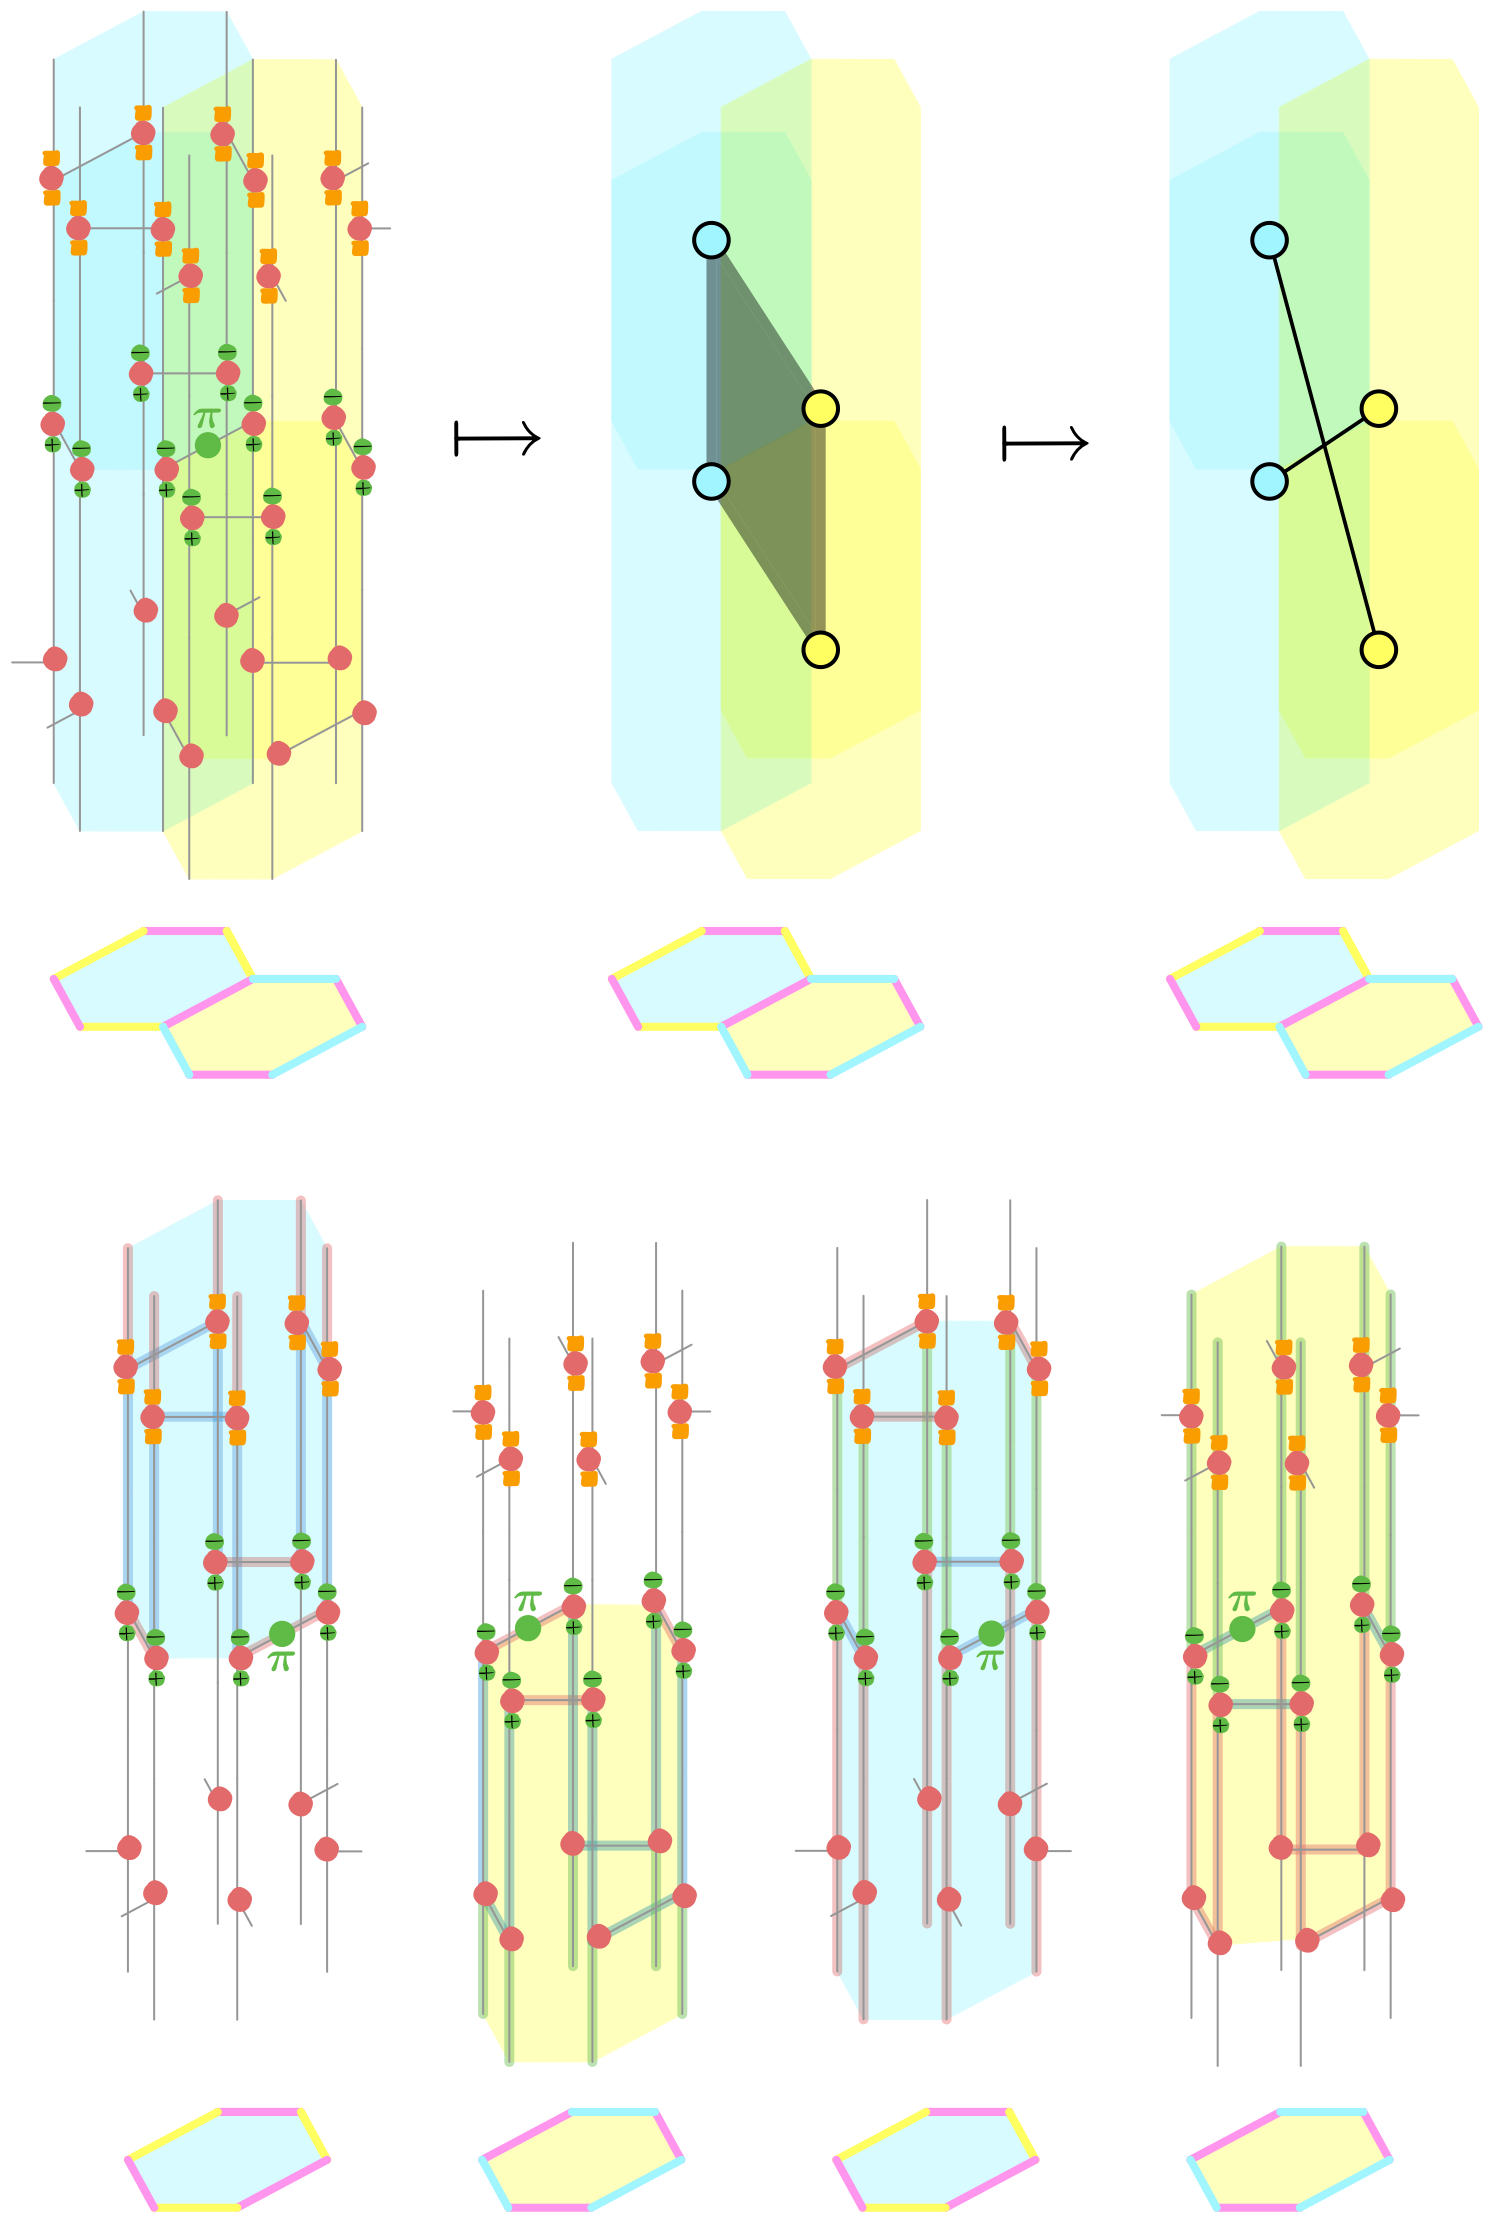
\includegraphics[width=0.8\textwidth]{figures/DCCCs/XYZ_measurement_error_hyperedge}
    \caption{
        An $e_{\textcolor{magenta}{m}, Y}$ measurement error in the $X^1Y^1Z^1$ honeycomb code, which violates four detectors.
        In the top left subfigure, we show the error as a ZX-diagram.
        Since it violates four detectors, it corresponds to a hyperedge in the decoding graph (top middle).
        This hyperedge then decomposes into two ordinary edges (top right).
        The longer of these two edges in the subfigure is a remnant edge,
        because there is no actual error in the noise model that corresponds to it,
        unlike the shorter of the two edges.
        The bottom subfigures show in more detail the four detectors that this error violates.
        One can check that these really are violated by noting that, in each case, the edge on which the green $\pi$-spider representing the error sits is highlighted a colour other than green,
        as explained in \Cref{fig:detectors_XYZ_and_CSS} and in more detail in \Cref{sec:zx-calculus-and-pauli-webs}.}
    \label{fig:XYZ_measurement_error}
\end{figure}

\begin{figure}[htb]
    \centering
    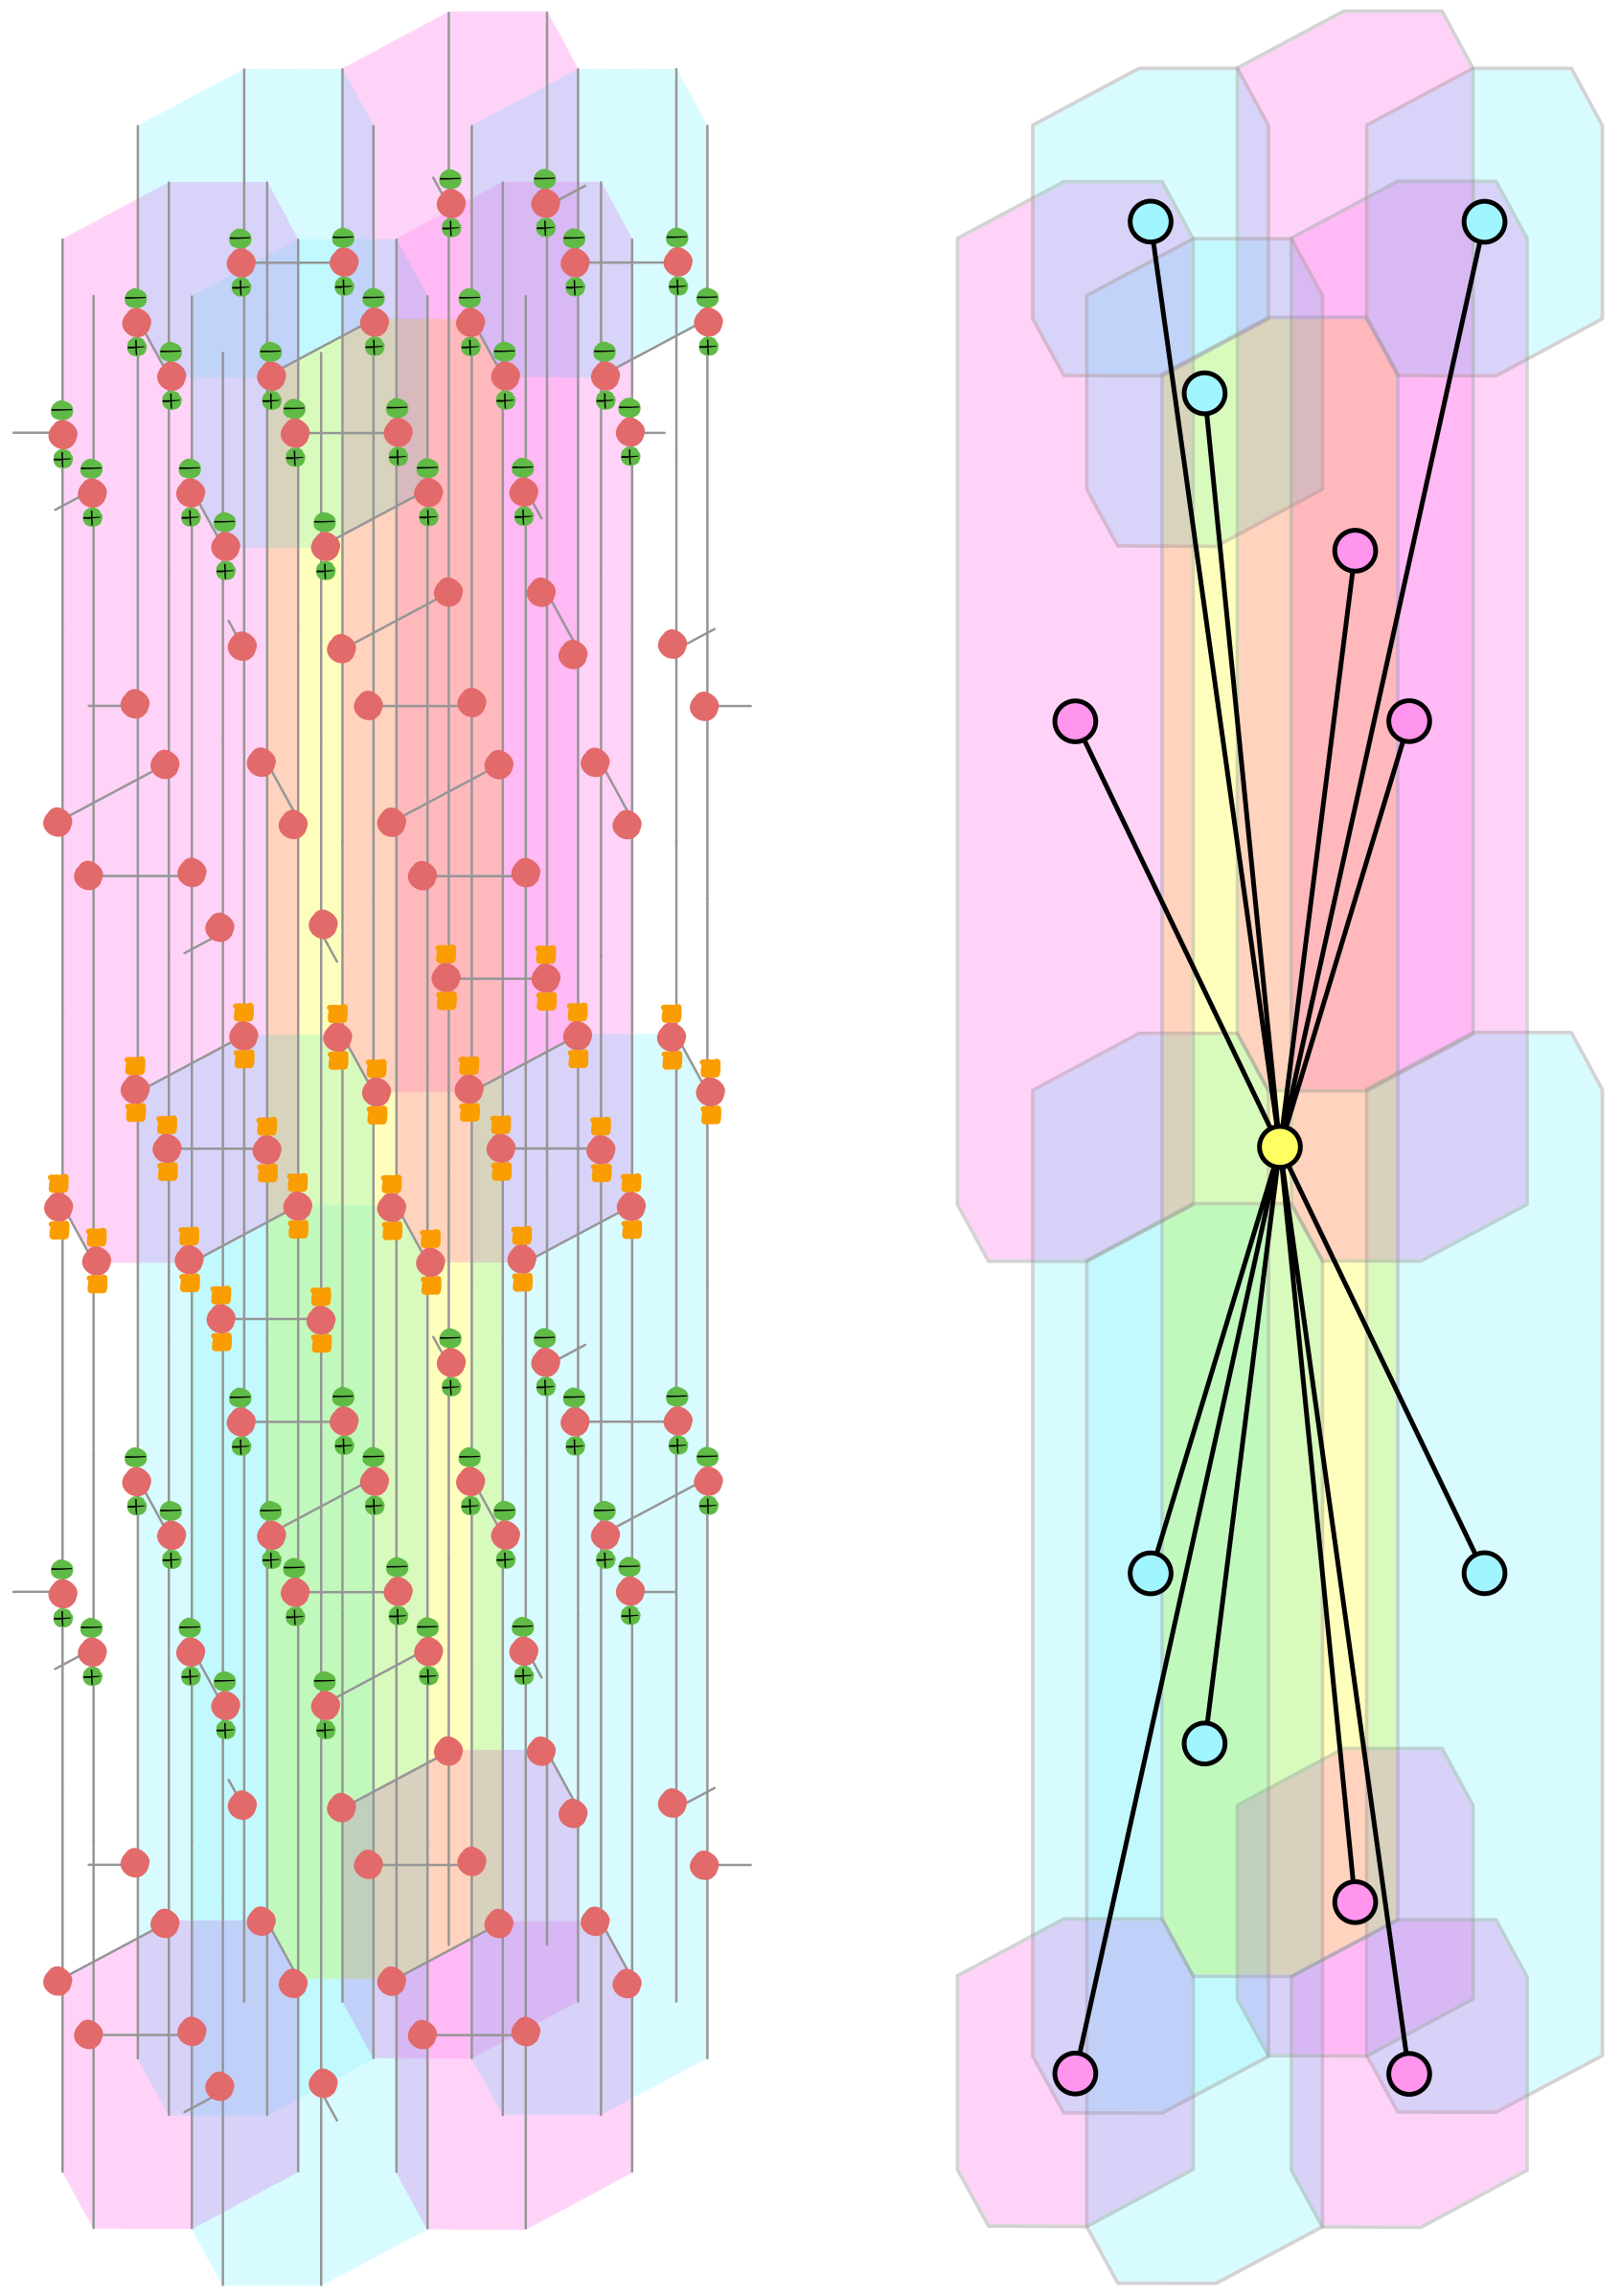
\includegraphics[height=0.55\textheight]{figures/DCCCs/decoding_graph_face_detector_neighbourhood}
    \caption{
        On the left we show five timesteps from the $X^1 Y^1 Z^1$ code.
        Areas coloured cyan, magenta and yellow denote detectors, though to make the diagram simpler we have not drawn the Pauli webs that define them (see \Cref{sec:detectors-cheatsheet} for a detector cheat sheet).
        On the right we show the neighbourhood of the yellow detector in the decoding graph, once all hyperedges have been decomposed into ordinary edges.
        This detector has degree 12, as does every other detector (apart from a few special cases right at the very start and end of the circuit).
        Crucially, this is also the case for the $X^1 Z^1$ code -- their decoding graphs after decomposition are isomorphic, differing only in the edge weights, i.e.\ in the probabilities of the corresponding errors occuring.}
    \label{fig:decoding_graph_face_detector_neighbourhood}
\end{figure}


The \textit{decoding graph} of a circuit implementing a quantum error-correcting code, under a given noise model, is a weighted hypergraph formed from the detectors of the code and the errors of the noise model.
The vertices of this hypergraph are exactly the detectors of the code.
For every possible independent error $e$ permitted by the noise model, letting $d_1, \ldots, d_b$ be the detectors it violates
and $p_e$ be the probability of it occurring,
a hyperedge also labelled $e$ is added to the graph, spanning vertices $\{d_1, \ldots, d_b\}$ and having weight $p_e$. 
As written, there may be multiple hyperedges spanning the same set of $\{d_1, \ldots , d_b\}$ of vertices;
if this is the case, they can be combined into a single hyperedge spanning this set of vertices,
whose weight $p$ is the probability of an odd number of the corresponding errors occurring.
We will alternatively write a hyperedge $e = \{d_1, \ldots, d_b\}$ as a formal product $e = d_1 \ldots d_b$ with powers mod 2.
As an example, in \Cref{fig:XYZ_measurement_error} we show a measurement error in the $X^1Y^1Z^1$ honeycomb code.
This violates four detectors, hence corresponds to a hyperedge spanning four vertices in the decoding graph\footnote{What we're calling a decoding graph is often called a \textit{Tanner graph}, though Tanner graphs are usually defined as bipartite graphs, with one type of vertex representing detectors, another type representing errors, and an edge between two vertices exactly if the corresponding error violates the corresponding detector. 
The two definitions are equivalent. The term \textit{detector error model} is also equivalently used \cite{gidney2022stim_error_model}.}.

Many of the best known decoding algorithms, however, can only be run on \textit{ordinary} graphs --
ones in which every hyperedge spans exactly $2$ vertices.
Decoders that require this form of graph are called \textit{matching decoders},
and include \textit{minimum-weight perfect matching} (MWPM) 
\cite{MWPM,dennis2002topological,MWPMColor}
and \textit{union-find} \cite{PhysRevResearch.2.033042,UnionFind}. 
We can transform the decoding graph into an ordinary graph, at the cost of the edge weights becoming only approximations of the corresponding errors occurring.

We start by `decomposing' errors that violate more than $2$ detectors into sets of errors that violate at most $2$ detectors.
For example, if the decoding graph contains a hyperedge $d_1 d_2 d_3 d_4$ with weight $p$,
but also a hyperedge $d_1 d_2$ with weight $p_{12}$ and a hyperedge $d_3 d_4$ with weight $p_{34}$,
then we can delete the hyperedge $d_1 d_2 d_3 d_4$ and update the weights $p_{12}$ and $p_{34}$ in some way.
In fact, even if the graph only contains hyperedges $d_1 d_2 d_3 d_4$ with weight $p$ and $d_1 d_2$ with weight $p_{12}$, 
we can delete $d_1 d_2 d_3 d_4$, update $p_{12}$ and add a new \emph{remnant edge} $d_3 d_4$ with some weight $p_{34}$.
In this work, we use the Clifford circuit simulator Stim~\cite{Gidney2021stimfaststabilizer} extensively,
and Stim's implementation of decomposing errors is described in \Ccite{stim_command_line_doc} and explained in \Ccite{gidney2022stim_error_model}.
The way in which the edge weights are updated is explained in Appendix C of \Ccite{higgott2022fragile}.
After decomposing all such hyperedges, we add a new virtual \emph{boundary vertex} $\partial$, and we replace every hyperedge spanning a single vertex $d$ with a new ordinary edge with endpoints $d$ and $\partial$ \cite{higgott2025sparse}.
At this point, every hyperedge will span exactly two vertices.

\subsection{Logical errors}\label{subsec:DCCCs_logical_errors}

If a set of errors do not violate any detectors,
but act non-trivially on the circuit implementing our code
(i.e.\ the circuit with errors is not equal as a linear map to the circuit without errors, even up to global scalar)
then this set constitutes a \textit{logical error}.
In a DCCC, we can further label logical errors as \textit{spacelike} or \textit{timelike}.
Intuitively, spacelike logical errors are those consisting of sets of errors wrapping around the torus on which the code is defined (in either direction).
Intuitively, timelike logical errors are those consisting of sets of errors that span from the start of the circuit to the end.
For example, if after some timestep $t$ a set of qubit errors occur whose tensor product is a logical Pauli operator for the code at this timestep $t$ -- like those depicted in \Cref{fig:logicals_XYZ_and_XZ} -- then this constitutes a spacelike logical error.
In \Cref{fig:XYZ_logical_data_qubit_errors}, we show one spacelike and one timelike logical error in the $X^1Y^1Z^1$ honeycomb code.

In any particular circuit and noise model,
the minimum number of errors required to create a logical error is defined to be the \textit{fault distance} of the circuit.
One can be more specific and speak of the \textit{spacelike fault distance} or \textit{timelike fault distance} --
the minimum number of errors required to create a spacelike or timelike logical error, respectively.
% Often we will refer to the \textit{distance} rather than the fault distance --
% this is just the fault distance in the specific case of the phenomenological noise model.


\begin{figure}[htpb]
    \centering
    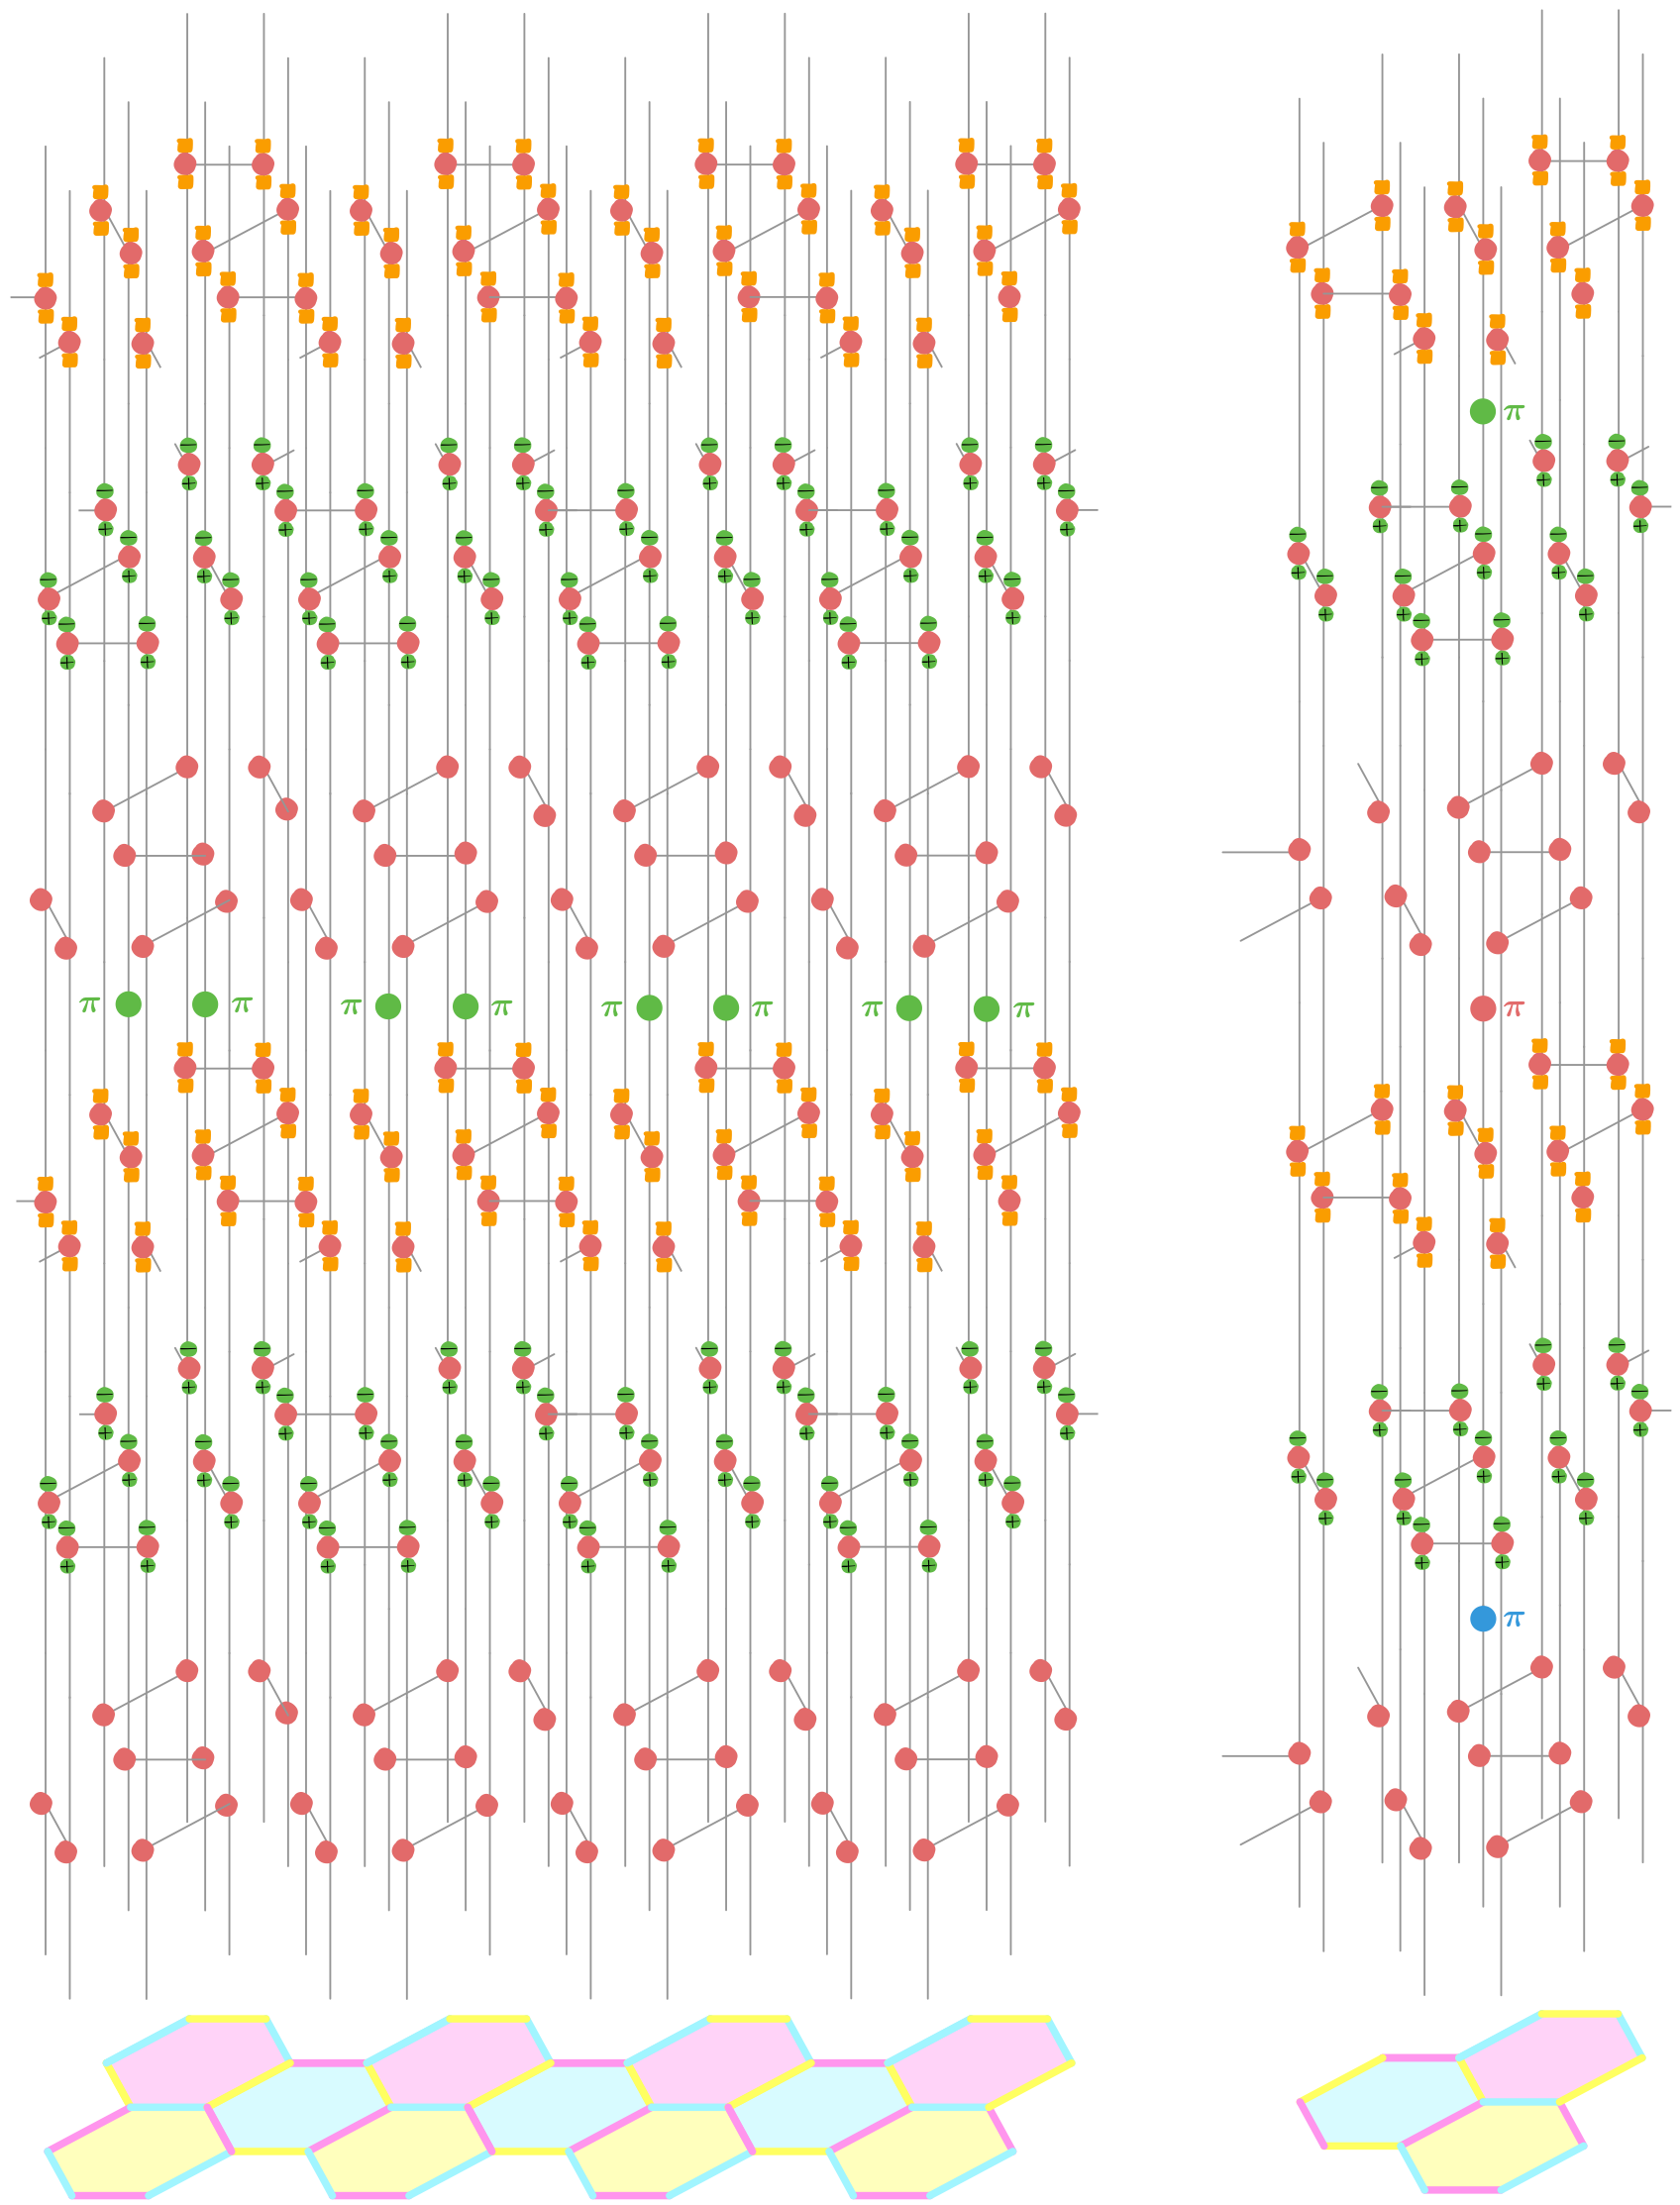
\includegraphics[width=\linewidth]{figures/DCCCs/XYZ_logical_data_qubit_errors}
    \caption{
        On a subset of qubits, we show a spacelike (left) and timelike (right) logical error in the XYZ honeycomb code consisting only of data qubit errors.
        \href{https://tinyurl.com/bdd7er9s}{Click here to view the spacelike} and 
        \href{https://tinyurl.com/ypwn6hca}{here to view the timelike} logical errors in
        Crumble~\cite{crumble}, a
        prototype tool for Clifford circuit exploration.}
\label{fig:XYZ_logical_data_qubit_errors}
\end{figure}

\subsection{Decoding}\label{subsec:decoding}

The decoding graph contains everything we need to be able to decode a quantum error-correcting code.
In general, decoding works as follows: as we run the circuit implementing the quantum error-correcting code,
we mark the vertices $d$ that correspond to violated detectors, then pass this marked graph to a decoder.
It is the job of the decoder to find a set of hyperedges (i.e., errors) satisfying two properties:
they could have caused these detectors to be violated,
and the combination of these errors and the actual errors that occurred do not constitute a logical error.
More precisely, let $e_1, \ldots, e_c$ be the actual errors that occurred,
which necessarily have formal product $e_1 \ldots e_c$ equal to the syndrome $d_1 \ldots d_b$.
The decoder's job is to find a set $e_1', \ldots, e_{c'}'$ of hyperedges such that the formal product $e_1' \ldots e_{c'}'$ is again $d_1 \ldots d_b$,
and the set of errors $\{e_1, \ldots, e_c, e_1', \ldots, e_{c'}'\}$ is not a logical error.

In this work, we consider two decoders: \textit{minimum-weight perfect matching (MWPM)} and \textit{belief matching}~\cite{higgott2022fragile}.
These are both matching decoders, so require the decoding graph to be an ordinary graph (or decomposable into an ordinary graph).
In MWPM, we simply apply the transformation described in \Cref{subsec:decoding_graph} to the decoding graph (i.e.~we convert the hypergraph into a graph).
Then, on any given run of the circuit, we apply the MWPM decoder to the resulting marked ordinary graph~\cite{higgott2025sparse}.
In belief matching, we add a pre-processing step which first adjusts the weights of the hyperedges in the marked decoding graph.
This pre-processing step is the classical decoding algorithm \textit{belief propagation} (BP)~\cite{McKay,Leifer,PhysRevResearch.2.043423}, which is run on the full decoding hypergraph to estimate the marginal probability of each error mechanism (whether it is an edge or hyperedge).
These marginal probabilities are then used to update the edge weights when converting to a graph for MWPM~\cite{higgott2022fragile}.
The details of exactly what this does are unimportant for us,
but the key intuition is that it recovers some of the information about the probabilities of errors occurring that's otherwise lost when transforming hyperedges into ordinary edges (i.e.~it exploits knowledge of the hyperedge errors when decoding a given syndrome).
This allows for more accurate decoding for error models containing hyperedges,
at the cost of slowing down the overall decoding process.
For those interested, a longer discussion of this trade-off can be found in \Ccite{higgott2022fragile}.
After running BP, we apply the transformation described in \Cref{subsec:decoding_graph} to the marked decoding graph,
and apply MWPM to the resulting marked ordinary graph.
A key line of investigation in this work is understanding for which DCCCs and noise models using belief matching brings most benefit.

\subsection{\texorpdfstring{$E$ and $M$ components}{E and M components}}\label{subsec:E_and_M_components}

In any DCCC, after applying the transformation described in \Cref{subsec:decoding_graph} to the decoding graph,
the new ordinary graph $G$ has the property that $G - \{\partial\}$ consists of two disconnected components,
where $\partial$ is the boundary vertex we added.
We will call one of these components the $E$ (electric) component and the other the $M$ (magnetic) component.
Then many of our other objects of interest inherit a label.
Detectors corresponding to vertices in the $E$ or $M$ component are labelled $E$ or $M$ detectors respectively.
Errors whose corresponding hyperedge in the original decoding graph spans vertices entirely in the $E$ or $M$ component of $G - \{\partial\}$
are labelled $E$ or $M$ errors, respectively.
Errors whose corresponding hyperedge spans vertices in both the $E$ and $M$ components are labelled $F$ (fermion) errors\footnote{%
    This $E$, $M$ and $F$ terminology is borrowed from the condensed matter approach, as in \Ccite{kesselring2022anyon}.
    We could equally have used the more standard $X$, $Z$ and $Y$ respectively, but we felt this could ultimately cause more confusion -- e.g. in the $X^1 Y^1 Z^1$ honeycomb code, some physical Pauli $X$ errors correspond to $E$ errors, some to $M$ errors, and some to $F$ errors.
    We felt it might be confusing to say that a Pauli $X$ error was actually a $Z$ error or a $Y$ error -- indeed, we confused ourselves many times in this project with this sort of terminology.}.
Spacelike logical errors that -- intuitively speaking -- wrap around the $E$ or $M$ component are labelled spacelike logical $E$ or $M$ errors respectively.
Timelike logical errors likewise inherit an $E$ or $M$ label.
Finally, the fault distances can be further divided into a spacelike $E$ and $M$ fault distance -- the minimum number of errors needed to create a spacelike logical $E$ or $M$ error, respectively -- and a timelike $E$ and $M$ fault distance -- the minimum number of errors needed to create a timelike logical $E$ or $M$ error, respectively.

\subsection{Boundaries}\label{subsec:boundaries}

As stated throughout this section, in this work we only consider DCCCs on a torus. Primarily, this is to make comparisons between different measurement schedules fair, since there are no boundaries at which they might behave differently. Helpfully, it also makes our analysis a great deal simpler. On the other hand, if one is ultimately interested in planar codes (e.g.\ because of hardware constraints) one might very reasonably question to what extent a code's performance in the toric setting is a good proxy for its performance in the planar setting.

First, we note that a general theory of boundaries for DCCCs is given in \Ccite[Section 7.3]{kesselring2022anyon}, so every DCCC can indeed be made planar. Furthermore, for the $X^1 Y^1 Z^1$ and $X^1 Z^1$ codes that we focus on in this work, specific boundaries are defined in \Ccite{gidney2022benchmarking} and \Ccite{kesselring2022anyon} respectively. In the former work, it's shown numerically that the planar $X^1 Y^1 Z^1$ code performs essentially as well as the toric version. In the latter work, no numerical results were given, but the detectors at the boundary were fully worked out and depicted. Since these follow exactly the same pattern as the detectors in the bulk, we again anticipate that performance of this planar $X^1 Z^1$ code would essentially mirror that of its toric counterpart, but have not verified this.
